\documentclass[letterpaper,10pt]{article}
\usepackage[utf8]{inputenc}

\usepackage{graphicx}
\usepackage{caption}
\usepackage{subcaption}
\usepackage{amsmath}
\usepackage{listings}
\usepackage[top=1in,bottom=1in,left=1in,right=1in]{geometry}

%opening
\title{Assignment 02 Report}
\author{Luke Fraser}


\begin{document}

\maketitle

\begin{abstract}
This assignment is centered around the use of image filtering. Image filtering can be used to perform many image processing operations. The term filtering comes from signal processing in which there are low-pass, high-pass, band-pass, and band-reject filters. Each filter provides different image results. The use of these image filters has implications far beyond just blurring images. The use of filters allows for smoothing, sharpening, data recovery, image derivatives, and much more. It is a useful tool to understand when working with images in general.
\end{abstract}

\section{Spatial Filtering}
Spatial filtering is used to perform many image processing operations. With spatial filtering you are able to perform filtering in relation to the frequency domain. You can also use image derivatives for edge detection. There are two central ways to perform filtering: convolution \& correlation. The two methods are very similar, but vary slightly in their definition. The two methods are very useful image processing operators when analyzing image data.	

\subsection{Correlation}
\begin{figure}[hbtp]
  \centering
  \begin{subfigure}{5cm}
    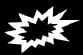
\includegraphics[width=5cm]{images/Pattern.png}
    \caption{Mask.}
  \end{subfigure}
  \begin{subfigure}{5cm}
    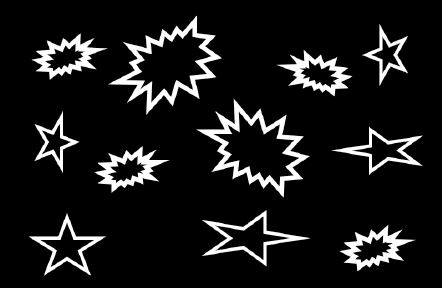
\includegraphics[width=5cm]{images/Image.png}
    \caption{Original Image.}
  \end{subfigure}
  \begin{subfigure}{5cm}
    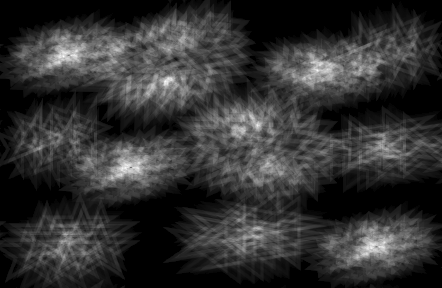
\includegraphics[width=5cm]{images/correlation.png}
    \caption{Correlation Image.}
  \end{subfigure}
  \label{fig:correlations}
\end{figure}

Correlation is an operation similar to the convolution and in many cases takes the place of the convolution in its implementation. Correlation as seen in the eq.~\ref{eq:correlation} uses a mask to compute the correlation on given image. As its name signifies Correlation is used to find where in an image a mask is similar. A high response from the correlation method signifies that a mask is present in the image. In this assignment we experimented with correlation to visually see how it could be used to register patterns in an image. As seen in Figure~\ref{fig:correlations} the mask was correlated with the original image to produce the resulting correlation image. It can be seen that there are high intensity ares of the image that signify a good match with the mask pattern. A serious limitation of this method is that it is not invariant to scale or orientation of the different patterns in the image. Meaning that only the patterns exactly aligned and sized correctly will respond strongly as matches.

\begin{equation}
g(x,y)=w(x,y)*f(x,y)=\sum_{s=-\frac{K}{2}}^{\frac{K}{2}}\sum_{t=-\frac{K}{2}}^{\frac{K}{2}}w(s,t)f(x+s,y+t)
\label{eq:correlation}
\end{equation}
\subsection{Smoothing}
  \begin{figure}[hbtp]
    \centering
    \begin{subfigure}{4cm}
      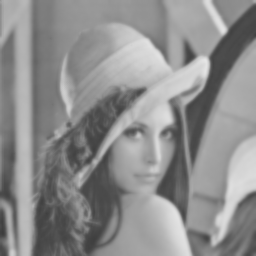
\includegraphics[width=4cm]{images/smoothing_gaussian_7.png}
      \caption{Kernel: 7x7 Gaussian.}
    \end{subfigure}
    \begin{subfigure}{4cm}
      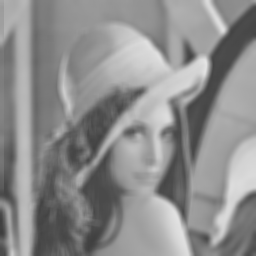
\includegraphics[width=4cm]{images/smoothing_average_7.png}
      \caption{Kernel: 7x7 Average.}
    \end{subfigure}
    \begin{subfigure}{4cm}
      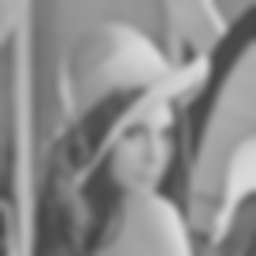
\includegraphics[width=4cm]{images/smoothing_gaussian_15.png}
      \caption{Kernel: 15x15 Gaussian.}
    \end{subfigure}
    \begin{subfigure}{4cm}
      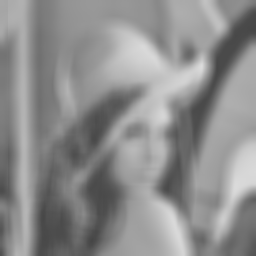
\includegraphics[width=4cm]{images/smoothing_average_15.png}
      \caption{Kernel: 15x15 Gaussian.}
    \end{subfigure}
    \caption{Image smoothing: A comparison between an average mask and a Gaussian mask.}
    \label{fig:smoothinglenna}
  \end{figure}
  \begin{figure}[hbtp]
    \centering
    \begin{subfigure}{4cm}
      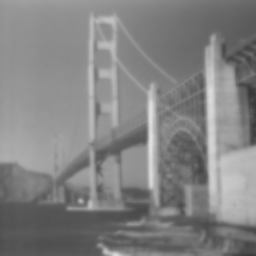
\includegraphics[width=4cm]{images/smoothing_sf_gaussian_7.png}
      \caption{Kernel: 7x7 Gaussian.}
    \end{subfigure}
    \begin{subfigure}{4cm}
      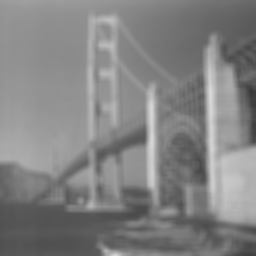
\includegraphics[width=4cm]{images/smoothing_sf_average_7.png}
      \caption{Kernel: 7x7 Average.}
    \end{subfigure}
    \begin{subfigure}{4cm}
      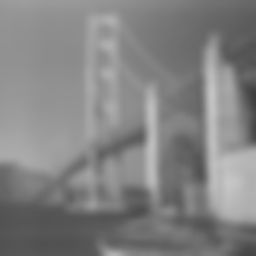
\includegraphics[width=4cm]{images/smoothing_sf_gaussian_15.png}
      \caption{Kernel: 15x15 Gaussian.}
    \end{subfigure}
    \begin{subfigure}{4cm}
      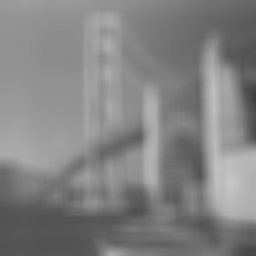
\includegraphics[width=4cm]{images/smoothing_sf_average_15.png}
      \caption{Kernel: 15x15 Gaussian.}
    \end{subfigure}
    \caption{Image smoothing: A comparison between an average mask and a Gaussian mask.}
    \label{fig:smoothingsf}
  \end{figure}
Smoothing is one of the most common operations performed on images to either remove noise and or sharpen features. Smoothing in the spatial domain is comparable to a low-pass filter in the frequency domain. eq~\ref{eq:convolution} shows the Gaussian distribution. Gaussian Smoothing is an important operation of image processing. It is one an can be used to smooth images in a unbiased fashion. Where as square masks when convolved with an image tend to leave behind traces of their shape. A Gaussian mask will not present artifacts in an image. Figure~\ref{fig:smoothinglenna} \&~\ref{fig:smoothingsf} show a comparison between average masks and Gaussian masks at different kernel sizes.
\begin{equation}
g(x,y)=w(x,y)*f(x,y)=\sum_{s=-\frac{K}{2}}^{\frac{K}{2}}\sum_{t=-\frac{K}{2}}^{\frac{K}{2}}w(s,t)f(x-s,y-t)
\label{eq:convolution}
\end{equation}
\begin{equation}
G_{\sigma}(x,y)=\frac{1}{2\pi \sigma^2}\mathrm{e}^{-\frac{x^2+y^2}{2\sigma^2}}
\label{eq:gaussian}
\end{equation}
\subsection{Sharpening}
\begin{figure}[hbtp]
    \centering
    \begin{subfigure}{4cm}
      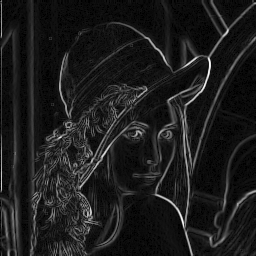
\includegraphics[width=4cm]{images/prewitt_lenna.png}
      \caption{Prewitt Magnitude.}
    \end{subfigure}
    \begin{subfigure}{4cm}
      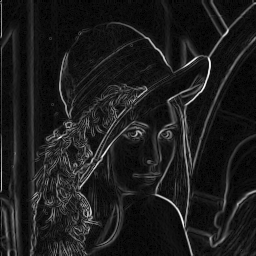
\includegraphics[width=4cm]{images/sobel_lenna.png}
      \caption{Sobel Magnitude.}
    \end{subfigure}
    \begin{subfigure}{4cm}
      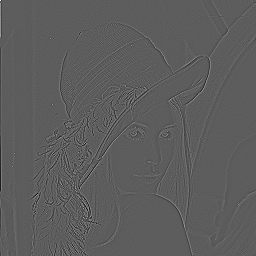
\includegraphics[width=4cm]{images/laplacian_lenna.png}
      \caption{Laplacian Mask.}
    \end{subfigure}
    \caption{Image Sharpening: Lenna.pgm sharpened using different mask operators.}
    \label{fig:sharpenlenna}
  \end{figure}
  \begin{figure}[hbtp]
    \centering
    \begin{subfigure}{4cm}
      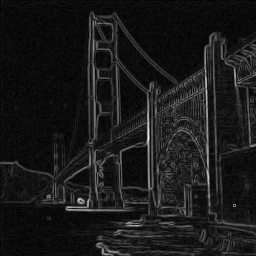
\includegraphics[width=4cm]{images/prewitt_sf.png}
      \caption{Prewitt Magnitude.}
    \end{subfigure}
    \begin{subfigure}{4cm}
      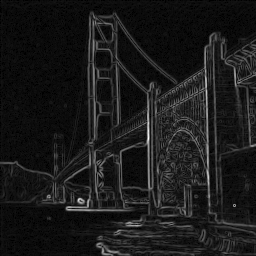
\includegraphics[width=4cm]{images/sobel_sf.png}
      \caption{Sobel Magnitude.}
    \end{subfigure}
    \begin{subfigure}{4cm}
      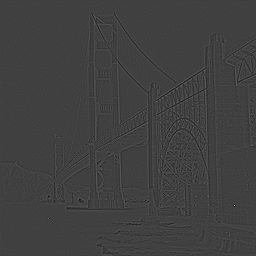
\includegraphics[width=4cm]{images/laplacian_sf.png}
      \caption{Laplacian Mask.}
    \end{subfigure}
    \caption{Image Sharpening: Lenna.pgm sharpened using different mask operators.}
    \label{fig:sharpensf}
  \end{figure}
Sharpening is used in image processing to emphasize high contrast details. In the case of the examples shown here image derivatives are taken to find the high contrast area. The use of the Sobel and Prewitt masks simulate image derivative to find lines in the image in both the x and y direction of the image. After each mask is convolved with the image you obtain the image gradient in both the x and y direction. To display the image results you compute the gradient magnitude to get a single number that represents the strength of the gradient in both directions. Figures~\ref{fig:sharpenlenna} \&~\ref{fig:sharpensf} show examples of the gradient magnitude taken with the sobel and prewitt masks.

The laplacian mask can also be used to find lines in images, but the line orientation is lost do to the method of the equation. The lapacian takes the second partial derivative in both directions of the image simultaneously. In the case of the Laplacian lines are located at the zero crossings in the resulting image. The results of all three masks are shown in Figures~\ref{fig:sharpenlenna} \&~\ref{fig:sharpensf}.
\section{Median Filtering}
\begin{figure}[hbtp]
  \centering
  \begin{subfigure}{4cm}
      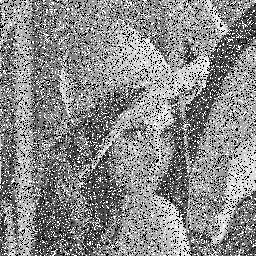
\includegraphics[width=4cm]{images/salt_lenna_30.png}
      \caption{Salt \& Pepper: 30.}
    \end{subfigure}
     \begin{subfigure}{4cm}
      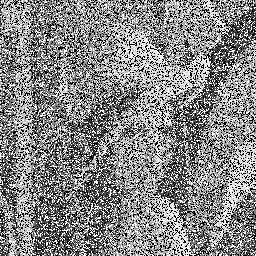
\includegraphics[width=4cm]{images/salt_lenna_50.png}
      \caption{Salt \& Pepper 50.}
    \end{subfigure}
    \caption{Salt \& Pepper Noise}
\end{figure}

 \begin{figure}[hbtp]
    \centering
    \begin{subfigure}{4cm}
      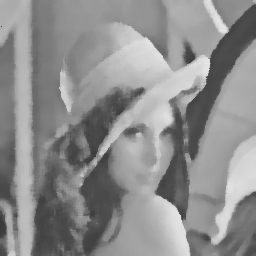
\includegraphics[width=4cm]{images/median_lenna_7.png}
      \caption{Kernel: 7x7 Noise: 30.}
    \end{subfigure}
    \begin{subfigure}{4cm}
      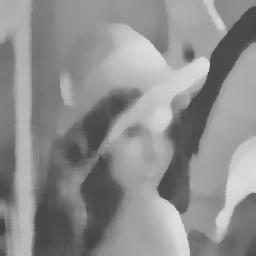
\includegraphics[width=4cm]{images/median_lenna_15.png}
      \caption{Kernel: 15x15 Noise: 30.}
    \end{subfigure}
    \begin{subfigure}{4cm}
      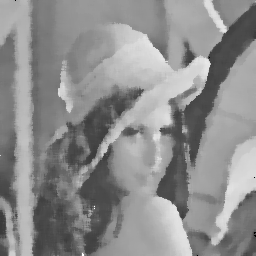
\includegraphics[width=4cm]{images/median_lenna_7_50.png}
      \caption{Kernel: 7x7 Noise: 50.}
    \end{subfigure}
    \begin{subfigure}{4cm}
      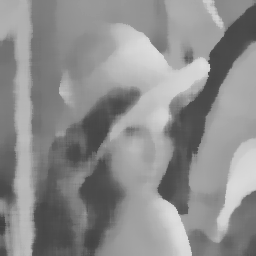
\includegraphics[width=4cm]{images/median_lenna_15_50.png}
      \caption{Kernel: 15x15 Noise: 50.}
    \end{subfigure}
    \caption{Median Filtering: Lenna.pgm.}
    \label{fig:medianlenna}
  \end{figure}
   \begin{figure}[hbtp]
    \centering
    \begin{subfigure}{4cm}
      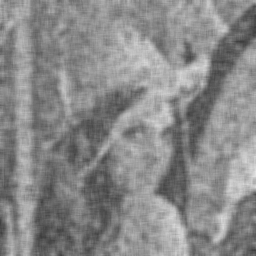
\includegraphics[width=4cm]{images/median_lenna_average_7_30.png}
      \caption{Kernel: 7x7 Noise: 30.}
    \end{subfigure}
    \begin{subfigure}{4cm}
      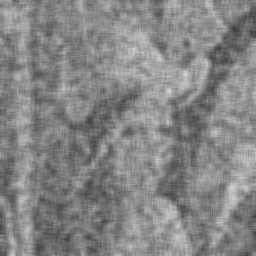
\includegraphics[width=4cm]{images/median_lenna_average_7_50.png}
      \caption{Kernel: 7x7 Noise: 50.}
    \end{subfigure}
    \begin{subfigure}{4cm}
      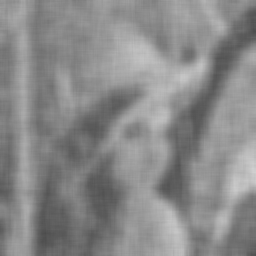
\includegraphics[width=4cm]{images/median_lenna_average_15_30.png}
      \caption{Kernel: 15x15 Noise: 30.}
    \end{subfigure}
    \begin{subfigure}{4cm}
      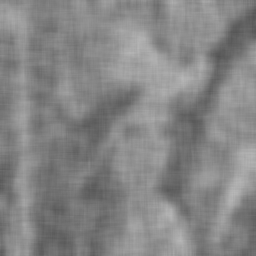
\includegraphics[width=4cm]{images/median_lenna_average_15_50.png}
      \caption{Kernel: 15x15 Noise: 50.}
    \end{subfigure}
    \caption{Average Filtering: Lenna.pgm.}
    \label{fig:averagelenna}
  \end{figure}
  \begin{figure}[hbtp]
    \centering
    \begin{subfigure}{4cm}
      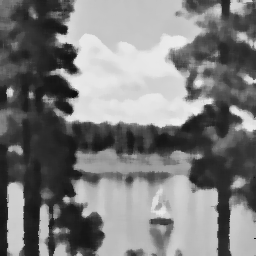
\includegraphics[width=4cm]{images/median_boat_7.png}
      \caption{Kernel: 7x7 Noise: 30.}
    \end{subfigure}
    \begin{subfigure}{4cm}
      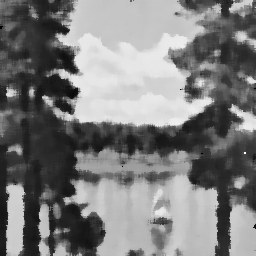
\includegraphics[width=4cm]{images/median_boat_7_50.png}
      \caption{Kernel: 7x7 Noise: 50.}
    \end{subfigure}
    \begin{subfigure}{4cm}
      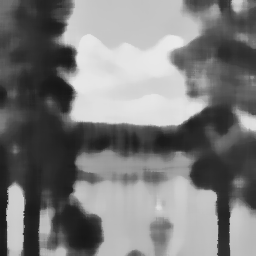
\includegraphics[width=4cm]{images/median_boat_15.png}
      \caption{Kernel: 15x15 Noise: 30.}
    \end{subfigure}
    \begin{subfigure}{4cm}
      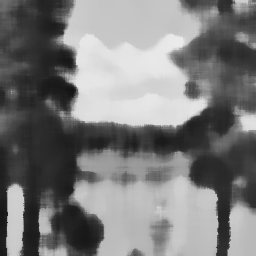
\includegraphics[width=4cm]{images/median_boat_15_50.png}
      \caption{Kernel: 15x15 Noise: 50.}
    \end{subfigure}
    \caption{Median Filtering: Boat.pgm.}
    \label{fig:medianboat}
  \end{figure}
   \begin{figure}[hbtp]
    \centering
    \begin{subfigure}{4cm}
      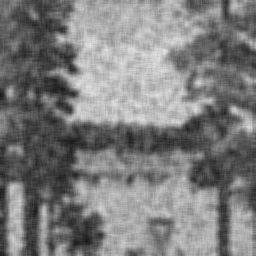
\includegraphics[width=4cm]{images/median_boat_average_7_30.png}
      \caption{Kernel: 7x7 Noise: 30.}
    \end{subfigure}
    \begin{subfigure}{4cm}
      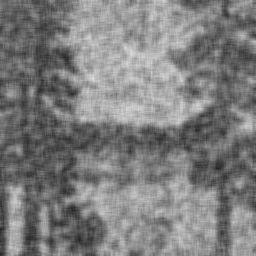
\includegraphics[width=4cm]{images/median_boat_average_7_50.png}
      \caption{Kernel: 7x7 Noise: 50.}
    \end{subfigure}
    \begin{subfigure}{4cm}
      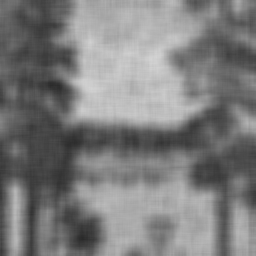
\includegraphics[width=4cm]{images/median_boat_average_15_30.png}
      \caption{Kernel: 15x15 Noise: 30.}
    \end{subfigure}
    \begin{subfigure}{4cm}
	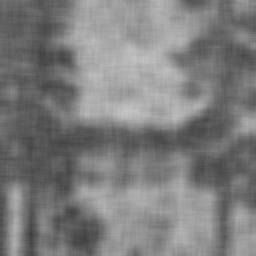
\includegraphics[width=4cm]{images/median_boat_average_15_50.png}
      \caption{Kernel: 15x15 Noise: 50.}
    \end{subfigure}
    \caption{Average Filtering: Boat.pgm.}
    \label{fig:averageboat}
  \end{figure}
Median Filtering is a filtering operation that unlike convolution and correlation does not sum the results of the mask. In the case of a median filter each element of the mask window is sorted into an ordered list where the median of the list is taken and used in the image in place of the previous pixel value. This filter has interesting effects on images and is well suited to remove noise in images. In the case of this example the results of a median filter on salt and pepper noise is shown in Figures~\ref{fig:medianlenna},~\ref{fig:averagelenna},~\ref{fig:medianboat},~\ref{fig:averageboat}.
\section{Unsharp Masking and High Boost Filtering}
  \begin{figure}[hbtp]
    \centering
    \begin{subfigure}{4cm}
      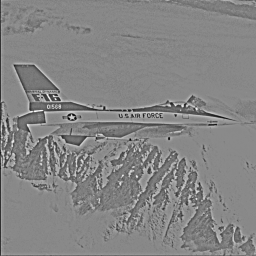
\includegraphics[width=4cm]{images/unsharp_highboost_f16_1-1.png}
      \caption{A=1.1}
    \end{subfigure}
    \begin{subfigure}{4cm}
      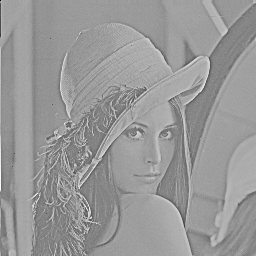
\includegraphics[width=4cm]{images/unsharp_highboost_lenna_1-3.png}
      \caption{A=1.3}
    \end{subfigure}
    \caption{Unsharp Masking and High Boost Filtering.}
    \label{fig:unsharp}
  \end{figure}
The Unsharp High boost filtering is combines several filtered images together to produce useful results. Equation~\ref{eq:highboost} shows the method used to generate the image in figure~\ref{fig:unsharp}. The Unsharp image is multiplied by a constant to reincorporate a portion of the original image back into the highpass image. The Highpass image is generated by taking the original image and subtracting a low pass filtered version of the image. This will produce a sharper highpass image. These to features come together to produce the resulting image in figure~\ref{fig:unsharp}.
\begin{equation}
 Highboost = (A-1)HighPass + Original - LowPass
 \label{eq:highboost}
\end{equation}

\end{document}

% Math equtions

% Forward Descrete Fourier transform
%F(u)=\frac{1}{N}\sum_{x=0}^{N-1}f(x)\mathrm{e}^\frac{-j2\pi ux}{N}{}, x = 0,1,...,N-1

% Inverse Descrete Fourier transoform
%f(x)=\frac{1}{N}\sum_{u=0}^{N-1}F(u)\mathrm{e}^\frac{j2\pi ux}{N}{}, x = 0,1,...,N-1

% Forward 2D Descrete Fourier transform
%F(u,v)=\frac{1}{N}\sum_{x=0}^{N-1}\sum_{y=0}^{N-1}f(x,y)\mathrm{e}^{-j2\pi\frac{ux+vy}{N}},(u,v) = 0,1,...,N-1

% Inverse 2D Descrete Fourier transform
%f(x,y)=\frac{1}{N}\sum_{u=0}^{N-1}\sum_{v=0}^{N-1}F(u,v)\mathrm{e}^{j2\pi\frac{ux+vy}{N}},(x,y) = 0,1,...,N-1

% Convolution
%g(x,y)=w(x,y)*f(x,y)=\sum_{s=-\frac{K}{2}}^{\frac{K}{2}}\sum_{t=-\frac{K}{2}}^{\frac{K}{2}}w(s,t)f(x-s,y-t)

% gradient
%\nabla f=\begin{pmatrix}\frac{\partial x}{\partial y} \\ \frac{\partial f}{\partial x} \end{pmatrix}

% Gaussian
%G_{\sigma}(x,y)=\frac{1}{2\pi \sigma^2}\mathrm{e}^{-\frac{x^2+y^2}{2\sigma^2}}
